%% grundlagen.tex
%% $Id: grundlagen.tex 28 2007-01-18 16:31:32Z bless $
%%

\chapter{Grundlagen}
\label{ch:Grundlagen}
%% ==============================

%% ==============================
\section{Kryptographie mit öffentlichen Schlüsseln}
%% ==============================
\label{ch:Grundlagen:sec:PublicKeyCrypto}

\subsection{Prinzip}
\label{ch:Grundlagen:sec:PublicKeyCrypto:subsec:Prinzip}

Klassische Kryptographie basiert auf einem \emph{Geheimnis} oder
\emph{privaten Schl\"ussel}, der beiden Kommunikationspartnern bekannt
ist. 

\subsection{Authentisierung von Schlüsseln}
\label{ch:Grundlagen:sec:PublicKeyCrypto:subsec:KeyAuth}

\subsubsection{Zentrale PKI}
\label{ch:Grundlagen:sec:PublicKeyCrypto:subsec:KeyAuth:subsubsec:PKI}

\subsubsection{Web of Trust}
\label{ch:Grundlagen:sec:PublicKeyCrypto:subsec:KeyAuth:subsubsec:WOT}

\section{PGP/GnuPG}
\label{ch:Grundlagen:sec:PGP}

\subsection{Geschichte von PGP und GnuPG}
\label{ch:Grundlagen:sec:PGP:subsec:Geschichte}

\subsection{Eigenschaften/Fähigkeiten der Implementierungen}
\label{ch:Grundlagen:sec:PGP:subsec:Eigenschaften}

\subsection{Das GnuPG-Vertrauensmodell}
\label{sec:das-gnupg-vertrauensmodell}

Öffentliche PGP-Schlüssel werden oft nicht in einer Weise übergeben,
die die sofortige Verifikation des Schlüssels zulässt, beispielsweise
bei einem persönlichen Treffen. Stattdessen werden Schlüssel häufig
per E-Mail, über einen Keyserver oder andere elektronische Wege
ausgetauscht.  Überprüfung der Authentizität eines Schlüssels ist
deswegen von grosser Bedeutung.

Ein Schlüssel wird von GnuPG genau dann als gültig (\emph{valid})
betrachtet, wenn er die folgenden Bedingungen erfüllt:

\begin{enumerate}
\item Der Schlüssel wurde von ausreichend vielen \emph{gültigen} Schlüsseln
  unterschrieben, d.h. er wurde mindestens entweder von
  \begin{itemize}
  \item dem Besitzer des Schlüsselrings selbst (d.h. von einem
    Schlüssel mit \emph{ultimate trust}) unterschrieben
  \item mindestens $N$ gültigen Schlüsseln, denen voll vertraut wird, unterschrieben
  \item mindestens $M$ gültigen Schlüsseln, denen geringfügig
    vertraut wird, unterschrieben
  \end{itemize}
\item Eine Signaturkette wird nur verwendet, wenn sie ausgehend vom
  Besitzer des Schlüsselrings maximal die Länge $L$ hat.
\end{enumerate}

Ein Schlüssel, der von weniger voll bzw. geringfügig
vertrauenswürdigen Schlüsseln als notwendig unterschrieben wurde, wird
als eingeschränkt gültig (\emph{marginally valid})
angesehen. Allerdings werden Schlüssel dieser Kategorie von GnuPG
genauso wie nicht gültige Schlüssel behandelt.

GnuPG verwendet in der Standardeinstellung die Werte $N=1$, $M=3$ und
$L=5$. Damit wird \emph{ein} Zertifikat, dass von einem Schl\"ussel
mit vollem Vertrauen ausgestellt wurde, als ausreichend
betrachtet. F\"ur Schl\"ussel, denen nur geringf\"ugig vertraut wird,
ist ein einzelnes Zertifikat nicht ausreichend. Dieses muss noch durch
2 weitere solche Zertifikate best\"atigt werden. 

GnuPG erlaubt es einem Anwender, die Parameter $N, M$ und $L$ selbst
zu setzen und damit seine Sicherheitsanforderungen umzusetzen. Je
höher beispielsweise die notwendige Anzahl von Signaturen, um so
kleiner ist der Schaden, den eine einzelne fehlerhafte Signatur
anrichten kann. Ist die maximale Pfadlänge auf einen kleinen Wert
begrenzt, so ist auch die maximale Anzahl der Signaturen auf dem Pfad
kleiner, die potentiell fehlerhaft sein können. Andererseits
verringert sich damit die Anzahl der Signaturen (Pfade im Web of
Trust), die für die Verifizierung benutzt werden können, und damit die
Anzahl verifizierbarer Schlüssel. Es muss also eine Abwägung zwischen
dem Sicherheitsbedürfnis des Nutzers und der praktischen Benutzbarkeit
getroffen werden.

\begin{figure}[t]
  \centering
  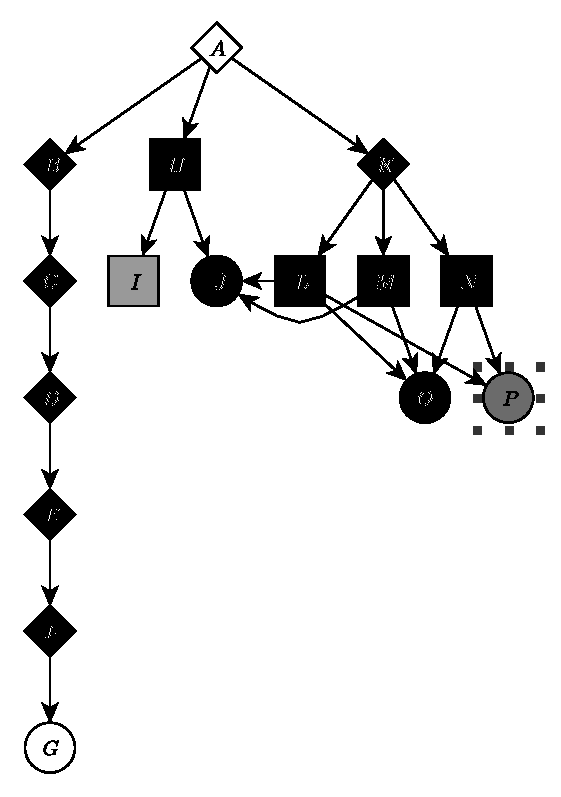
\includegraphics[scale=1.0]{images/trust-beispiel.pdf}
  \caption{Beispiel für die Berechnung der Gültigkeit von Schlüsseln}
  \label{fig:trust-beispiel}
\end{figure}

Abbildung \ref{fig:trust-beispiel} gibt ein Beispiel für die
Berechnung der Schlüsselgültigkeit unter Verwendung der
Standard-Parameter $N=1$, $M=3$ und $L=5$. Die Schlüssel $B, H$ und
$K$ wurden direkt von $A$, dem Besitzer des Schlüsselrings,
unterschrieben und sind deshalb voll gültig. Da $L, M,$ und $N$ von
$K$ unterschrieben wurden und dieser über volles Vertrauen verfügt,
sind sie ebenfalls voll gültig. $O$ sowie $J$ sind voll gültig, da sie
jeweils von drei Schlüsseln mit geringfügigem Vertrauen unterschrieben
wurden. $I$ und $P$ wurden dagegen jeweils nur von zwei Schlüsseln mit
geringfügigem Vertrauen unterschrieben und sind deshalb nicht voll
sondern nur eingeschränkt gültig. $G$ wurde zwar von einem voll
gültigen Schlüssel mit vollem Vertrauen unterschrieben. Allerdings
überschreitet die Signaturkette zu $A$ die maximale Länge von 5 und
wird deshalb nicht betrachtet.



Ein öffentlicher Schlüssel, der anhand dieser Regeln nicht als
authentisch verifiziert werden kann, kann trotzdem zur Verschlüsselung
und zur Verifizierung von Signaturen verwendet werden. Allerdings
warnt GnuPG in diesem Fall vor der Verwendung.

\subsection{Soziale Komponente des Web of Trust}
\label{sec:sozi-komp-des}



%% ==============================
\section{Der OpenPGP-Standard (RFC4880)}
%% ==============================
\label{ch:Grundlagen:sec:OpenPGP}

\subsection{Paketformat v4}
\label{ch:Grundlagen:sec:OpenPGP:subsec:PaketFormat}

\subsection{Unterschiede v3}
\label{ch:Grundlagen:sec:OpenPGP:subsec:v3Format}

\section{Graphentheorie allgemein}
\label{ch:Grundlagen:sec:Graphentheorie}

\section{Netzwerkanalyse}
\label{ch:Grundlagen:sec:Netzwerkanalyse}

\subsection{Netzwerkstatistiken}
\label{ch:Grundlagen:sec:Netzwerkanalyse:subsec:Statistiken}

\subsection{Communities}
\label{ch:Grundlagen:sec:Netzwerkanalyse:subsec:Communities}

Seit der Arbeit von Newman wurde eine Vielzahl weiterer Methoden zur
Erkennung von Communities vorgestellt. An dieser Stelle werden 3
Methoden n\"aher beschrieben, die in dieser Arbeit verwendet
werden. Einen Gesamt\"uberblick bietet ein \"Ubersichtsartikel von
Fortunato \cite{Fortunato2010}.




%% ==============================
\section{Verwandte Arbeiten}
%% ==============================
\label{ch:Grundlagen:sec:RelatedWork}

\subsection{Analysen des OpenPGP-Web of Trust}
\label{ch:Grundlagen:sec:RelatedWork:subsec:wot-analysis}

\subsection{Community-Strukturen allgemein}
\label{ch:Grundlagen:sec:RelatedWork:subsec:community-analysis}

In Abschnitt \ref{sec:sozi-komp-des} wurden Mechanismen beschrieben,
die zur Entstehung des Web of Trust beitragen. Ausgehend davon kann
die Annahme getroffen werden, dass die Vernetzung wesentlich von zwei
Faktoren beeinflusst wird: Teilnehmer vernetzen sich einerseits
aufgrund ihrer Zugeh\"origkeit zu einer \emph{sozialen Gruppe}. Dabei
kann es sich um Open-Source-Projekte wie z.B. Debian, akademische
Einrichtungen und Firmen handeln, aber auch um eine Gruppe von
Freunden oder Bekannten. Andererseits vernetzen sich Teilnehmer auf
Keysigning-Parties mit einer relativ grossen Anzahl Benutzer, die
ihnen nicht unbedingt bekannt sind und mit denen sie keine starke
Gruppenzugeh\"origkeit verbindet. Offensichtlich ist allerdings, dass
diese 

Es soll nun untersucht werden, inwiefern sich diese postulierten
Entstehungsmechanismen in der Struktur des Web of Trust
wiederfinden. Angenommen wird, dass sich ein hoher Anteil der
Teilnehmer prim\"ar anhand dieser beiden Mechanismen vernetzen und der
Anteil an Signaturen zwischen Teilnehmern, die nicht durch eine
Keysigning-Party oder eine soziale Gruppe entstanden ist, deutlich
geringer ist. In diesem Fall ist zu erwarten, dass sich soziale
Gruppen und die Ergebnisse von Keysigning-Parties als Gruppen von
Knoten im Netzwerk wiederfinden, die untereinander eine hohe Anzahl
von Kanten hat, d.h. \emph{dicht} vernetzt ist, w\"arend sich zu
Knoten ausserhalb der Gruppe nur relativ wenige Kanten finden. Diese
Eigenschaft entspricht exakt der in Abschnitt
\ref{ch:Grundlagen:sec:Netzwerkanalyse:subsec:Communities}
beschriebenen Definition von \emph{Communities}. Es erscheint als
Methode deshalb sinnvoll, mit vorhandenen Methoden zur
Community-Erkennung eine Zerlegung des Graphen zu berechnen und dann
zu untersuchen, inwiefern sich die einzelnen so berechneten
Communities entsprechend der Annahme auf soziale Gruppen
bzw. Keysigning-Parties abbilden lasse.

Dazu sind Kriterien n\"otig, um eine berechnete Community einer
sozialen Gruppe, einer Keysigning-Party oder beidem zuzuordnen. F\"ur
Keysigning-Parties ist anzunehmen, dass die Signaturvorg\"ange
zwischen den Teilnehmern einer KSP innerhalb eines eng begrenzten
Zeitraums nach Stattfinden der KSP vorgenommen werden. Als einfaches
Kriterium f\"ur die Erkennung einer Keysigning-Party kann also eine
starke zeitliche Korrelation der Signaturvorg\"ange zwischen der
Mehrzahl der Community-Mitglieder verwendet werden. Konkret wird hier
eine Community als Produkt einer KSP betrachtet, wenn 80\% der
Signaturen zwischen den Mitgliedern innerhalb eines Monats vorgenommen
wurden.

Die Zuordnung zu sozialen Gruppen wird dadurch erschwert, dass --
abgesehen von den Schl\"usseln und Signaturen selbst -- keine
empirischen Daten \"uber die Gruppenzugeh\"origkeit vorliegen. Die
einzigen Daten, die eine (primitive) Zuordnung erlauben, sind die in
den UserIDs enthaltenen E-Mail-Adressen. \"Uber die Top-Level-Domain
(TLD) kann ein User einem Land zugeordnet werden, sofern es sich nicht
um eine der generischen TLDs (com, org, net) handelt. \"Uber die
Second-Level-Domain kann versucht werden, einen Nutzer einer
Institution zuzuordnen. Ein User, der beispielsweise \"uber eine
E-Mail-Adresse mit der Domain debian.org verf\"ugt, ist sicherlich ein
Mitglied des Debian-Projekts. Hilfreich dabei ist, dass Teilnehmer
dazu tendieren, alle ihre Adressen auf ihren Schl\"usseln zu
vermerken, so dass viele Schl\"ussel mehrere UserIDs und
E-Mail-Adressen haben (siehe Abschnitt
\ref{sec:result-key-properties}). Dadurch werden die verf\"ugbaren
Informationen \"uber Gruppenzugeh\"origkeiten erh\"oht. Adressen
verbreiteter ``Freemail-Anbieter'' wie Gmail, GMX und Yahoo sowie
Adressen von Internet Service Providern d\"urfen dabei nat\"urlich
nicht verwendet werden, weil ihre Verwendung nichts \"uber eine
Gruppenzugeh\"origkeit aussagt.

Die Schwellwerte wurden nicht anhand empirischer Daten festgelegt
sondern dr\"ucken nur ein intuitives Verst\"andnis f\"ur die
\"uberwiegende Mehrzahl der Mitglieder einer Gruppe bzw. die einen
erheblichen Anteil der Mitglieder einer Gruppe aus.


%%% Local Variables: 
%%% mode: latex
%%% TeX-master: "diplarb"
%%% End: 
